% Template for Cogsci submission with R Markdown

% Stuff changed from original Markdown PLOS Template
\documentclass[10pt, letterpaper]{article}

\usepackage{cogsci}
\usepackage{pslatex}
\usepackage{float}
\usepackage{caption}

% amsmath package, useful for mathematical formulas
\usepackage{amsmath}

% amssymb package, useful for mathematical symbols
\usepackage{amssymb}

% hyperref package, useful for hyperlinks
\usepackage{hyperref}

% graphicx package, useful for including eps and pdf graphics
% include graphics with the command \includegraphics
\usepackage{graphicx}

% Sweave(-like)
\usepackage{fancyvrb}
\DefineVerbatimEnvironment{Sinput}{Verbatim}{fontshape=sl}
\DefineVerbatimEnvironment{Soutput}{Verbatim}{}
\DefineVerbatimEnvironment{Scode}{Verbatim}{fontshape=sl}
\newenvironment{Schunk}{}{}
\DefineVerbatimEnvironment{Code}{Verbatim}{}
\DefineVerbatimEnvironment{CodeInput}{Verbatim}{fontshape=sl}
\DefineVerbatimEnvironment{CodeOutput}{Verbatim}{}
\newenvironment{CodeChunk}{}{}

% cite package, to clean up citations in the main text. Do not remove.
\usepackage{cite}

\usepackage{color}

% Use doublespacing - comment out for single spacing
%\usepackage{setspace}
%\doublespacing


% % Text layout
% \topmargin 0.0cm
% \oddsidemargin 0.5cm
% \evensidemargin 0.5cm
% \textwidth 16cm
% \textheight 21cm

\title{Drawings as a window into object representations in childhood}


\author{{\large \bf Bria Long} \\ \texttt{bria@stanford.edu} \\ Department of Psychology \\ Stanford University \And {\large \bf Judy Fan} \\ \texttt{jefan@stanford.edu} \\ Department of Psychology \\ Stanford University \And {\large \bf Michael C. Frank } \\ \texttt{mcfrank@stanford.edu} \\ Department of Psychology \\ Stanford University}

\begin{document}

\maketitle

\begin{abstract}
A few well placed strokes can convey the identity of a person, object,
or place. How do we become so skilled at creating these graphical
abstractions? Here, we take a developmental appraoch to question by
asking children (age range 3-10 years) to draw a wide range of objects
(e.g. `can you draw a chair?'). First, we analyze the degree to which
children were able to depict recognizable exemplars of these categories
in under 30 seconds. We find that children become increasingly skilled
at producing recognizable drawings, even when controlling for low-level
covariates (the amount of ink used, the time spent drawing, and the
number of strokes). Second, we analyze the degree to which children's
drawings share perceptual features with those produced by adults by
analyzing their featural similarity at each layer of deep convolutional
neural network (VGG-19). Overall, we find that older children's drawings
were most similar to adults in higher-levle layers of the network, while
younger childrens drawings were most similar to adults in mid-level
layers of the network. Thus, these results suggest that the ability to
produce abstract graphical represnetations of objects is highly
developed by middle childhood, but that even the most primitive drawings
made by children contain featural similarities to the objects they are
trying to depict. Broadly, these results point towards drawing as a
promising avenue for investigating object representations in childhood.

\textbf{Keywords:}
object representations; drawings; child development
\end{abstract}

\section{Introduction}\label{introduction}

Consider what one has to do in order to draw ``a phone'' -- one needs to
access a the mental representation of ``a phone'', distill this into a
pictoral format, and plan a sequence of motor actions to effectively
convey this visual concept. Yet this is a trivial task for ordinary
adults. How do we learn to so effectively produce recognizable drawings?
And might drawings offer a window into how young children represent
common object categories?

While drawing has been extensively studied in early childhood, a primary
focus has been on when children come to treat drawings as symbols for
object categories (Gardner, 1994). And a wealth of evidence now suggests
that in fact young children attribute rich meanings to their drawings.
For example, children will attribute different symbolic content (e.g.,
``a balloon'', ``a lollipop'') to very similar drawings based on what
they intended to draw (Bloom \& Markson, 1998). Further, children will
monitor whether their drawings are adequate symbols for the things they
are trying to draw, and will improve their drawings when given feedback
that their drawings are not effective at communicating the identity of
object (Callaghan, 1999).

Far less research, however, has examined how children's drawings reflect
how children represent objects in the world around them. Indeed,
drawings are a powerful way to tap internal representations of object
categories, even in non-expert adults. For example, adults tend to draw
objects that are small in the real-world at small visual sizes, and
objects that are big in the real-world at big visual sizes (Konkle \&
Oliva (2011)). Further, to be recognizable, drawings have to depict the
necessary features to express a given visual concept. This intuition is
supported by recent computational work: deep neural network models of
the ventral stream trained purely on photographs can also recognize
drawings by non-expert adults, as drawings and photographs generated
similar representations in higher-level layers of these models. In other
words, drawings capture high-level similarity relationships between
object categories (Fan, Yamins, \& Turk-Browne, 2015).

Here, we explore how children draw common object categories across early
childhood. First, we ask if children produce more recognizable drawings
as they get older after factoring out low-level covariates. Second, we
examine the degree to which children produce drawings that contain
similar perceptual features characteristic of common object categories
by comparing their children and adult's drawings at each layer of a deep
convolutional neural network.

\section{Part 1: Why do children get better at
drawing?}\label{part-1-why-do-children-get-better-at-drawing}

First, children across a wide range of ages produced drawings of 16
common object categories in a simple drawing game. Then, naïve adults
attempted to recognize these drawings in a forced-choice recognition
task.

\subsection{Methods}\label{methods}

\subsubsection{Participants}\label{participants}

For the drawing task, children (N = 41, M = 6.9 years, range 4-10 years)
were recruited at the San Jose Children's Discovery Museum and
participated in this experiment. For the recognizability experiment, 14
adults with US IP addresses were recruited and rated all of the 268
drawings.

\subsubsection{Materials}\label{materials}

We implemented a simple drawing game in HTML/Javascript using the
paper.js library; this web-based experiment was run on an iPad on the
floor of the museum. All code is available at
www.github.com/brialorelle/kiddraw/museumdraw.

\subsubsection{Drawing Game Procedure}\label{drawing-game-procedure}

On each trial, a text cue would appear (i.e., ``Can you draw a
{[}dog{]}?'') that the experimenter would read out, (``What about a
{[}dog{]}? Can you draw a {[}dog{]}?). Then, a drawing canvas appeared
(600 x 600 pixels) and children were had 30 seconds to make a drawing
before the game moved on to the next trial. After each trial, the
experimenter asked the child whether they wanted to keep drawing or
whether they were all done. On the first two trials of the experiment,
every child was prompted to draw the same two common shapes----a circle
and a triangle. These trials served to familiarize children with the
drawing task and to practice using their fingers to draw.

\subsubsection{Stimuli}\label{stimuli}

Stimuli were words referring to 16 common object categories (banana,
boat, car, carrot, cat, chair, couch, cup, flower, foot, frog, ice
cream, phone, rabbit, shoe, train). These categories were chosen such
that they were (1) likely to be familiar to children, (2) present in the
Google QuickDraw database, (3) spanned the animate/inanimate distinction
and (4) intuitively spanned a wide range of difficulty (for example,
flowers seem easier to draw than couches).

\subsubsection{Recognizability Task}\label{recognizability-task}

14 naïve adults assessed the recognizability of all of the 286 drawings
produced by these children. On each trial, participants saw a drawing,
and were asked ``What does this look like?'', and responded by typing
into a text box; participants could then choose between 21 possible
answers. 16 of these possible answers were the original object
categories; however, we also included five additional foil items (bean,
arm, person, rock, and ``cannot tell at all''). All drawings were
presented in a random order, and participants were not informed that
these drawings were produced by children or the context in which they
were produced. An answer was scored as ``correct'' if adults were able
to correctly guess the object category that children were cued with.

\begin{CodeChunk}
\begin{figure*}[h]

{\centering 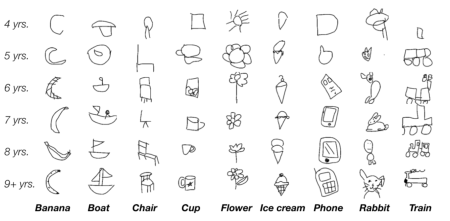
\includegraphics[width=1\linewidth]{figs/exampleDrawings-1} 

}

\caption[Example drawings made by children ages 4-10 of several object  categories]{Example drawings made by children ages 4-10 of several object  categories.}\label{fig:exampleDrawings}
\end{figure*}
\end{CodeChunk}

\subsubsection{Low-level covariates.}\label{low-level-covariates.}

The use of a digital interface for drawing allowed us to quickly and
easily assess the contribution of several low-level factors that may
co-vary with drawing ability. For each drawing, we thus quantified the
amount of time spend drawing, the number of strokes used, and the
overall intensity of the drawing(e.g., amount of ink). Descriptives
plots describing the output of these variables can be seen in (see
Figure \ref{fig:covDescriptives}, left).

\begin{CodeChunk}
\begin{figure*}[h]

{\centering 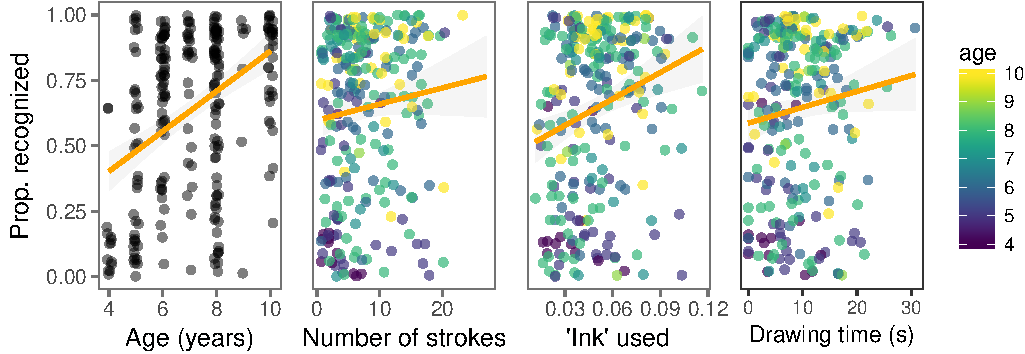
\includegraphics{figs/covDescriptives-1} 

}

\caption[The proportion of adults who recognized each drawing is plotted as a function of the number of strokes, amount of ink used, and the time spent creating each drawing]{The proportion of adults who recognized each drawing is plotted as a function of the number of strokes, amount of ink used, and the time spent creating each drawing. Each dot represents an individual drawing; dots are colored by the age of the drawer.}\label{fig:covDescriptives}
\end{figure*}
\end{CodeChunk}

\subsubsection{GLMM procedure.}\label{glmm-procedure.}

We aimed to assess whether children's ability to produce recognizable
drawings increased with age, independent of low-level covariates. To do
so, we used a generalized logistic mixed effect model, with age, drawing
duration, amount of ink used, and number of strokes as fixed effects,
and with random effects for each individual child drawer and object
category.

\subsection{Results}\label{results}

First, we observed that some items were much easier to draw than others.
For example, children of all ages produced drawings of cats that were
readily recognizable as ``cats'', but few children of any age produced
drawings that were recognizable as ``shoes'' (see Figure
\ref{fig:recognizabilityByItem}). Howver, almost all items also saw an
increase in recognizability with the age of the drawer. Across all
items, the proportion of drawings recognized increased steadily with age
(\% drawings recognized; chance = 4.8\%; \(M_{4yrs}\) = 14\%,
\(M_{5yrs}\) = 45\%, \(M_{6yrs}\) = 70\%, \(M_{7yrs}\) = 72\%,
\(M_{8yrs}\) = 66\%, \(M_{9yrs}\) = 76\%, \(M_{10yrs}\) = 85\%).

Next, we asked whether this relationsip persists when we control for
low-level covariates: the number of strokes, amount of ink used, and the
time spent drawing. In other words, is this increase in recognizability
due to an increase in expressive power, or simply due to the fact that
older children may have put more effort into their drawings? Our
generalized logistic mixed-effect model revealed that the
recognizability of drawings increased reliably with when controlling for
these low-level covariates --- the amount of time spent drawing, the
number of strokes, and total ink used (b = 0.96, SE = 0.17, Z = 5.5),
and accounting for variation across object categories and individual
children. All model coefficients can be seen in Table
\ref{table:modelCoefficients}. Adding interaction terms between age and
these low-level covariates did little to decrease the effect of age on
recognizability (b = 0.94, SE = 0.18, Z = 5.4).

Thus, these results suggest that the ability to quickly produce
graphical representations of object categories increases with age,
independently of low-level covariates. Further, these results sugest
that this ability is highly developed by middle childhood, plateauing
for these object cateogries around age 6-7.

\begin{CodeChunk}
\begin{figure}[H]

{\centering 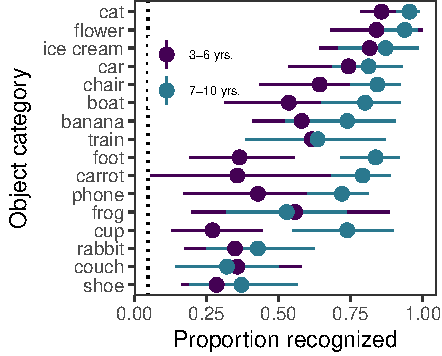
\includegraphics{figs/recognizabilityByItem-1} 

}

\caption[Proportion of drawings recognized for object category, sorted from hardest to easiest items]{Proportion of drawings recognized for object category, sorted from hardest to easiest items. Error bars represent non-parametric 95 percent confidence intervals, estimated using the langcog r package.}\label{fig:recognizabilityByItem}
\end{figure}
\end{CodeChunk}

\begin{table}[H]
\centering
\begin{tabular}{rrrrr}
  \hline
 & Estimate & Std. Error & z value & Pr($>$$|$z$|$) \\ 
  \hline
(Intercept) & 0.861 & 0.321 & 2.680 & 0.007 \\ 
  Age & 0.956 & 0.174 & 5.497 & 0.000 \\ 
  Drawing time & 0.338 & 0.109 & 3.105 & 0.002 \\ 
  Amount of ink & 0.014 & 0.080 & 0.179 & 0.858 \\ 
  Num. strokes & -0.289 & 0.098 & -2.959 & 0.003 \\ 
   \hline
\end{tabular}
\caption{Model coefficients of a GLMM predicting the recognziability of each  drawing.} 
\end{table}

\section{Part 2: How similar are children's and adults'
drawings?}\label{part-2-how-similar-are-childrens-and-adults-drawings}

To what degree are children's drawings similar to those of adults? While
younger children often produced drawings that were unrecognizable at the
basic-level, these recognizability ratings may underestimate the
perceptual content depicted in children's drawings. For example,
children may not be able to depict the visual differences between a
bunny and a frog, but they still may capture many of the essential
perceptual features needed to depict an animal. Here, we turn to deep
neural network models of object recognition to quantify the similarities
between children's and adults drawings, asking how similar they are in
terms of feature similarity at each progressively complex layer of a
deep convolutional neural network. While younger and older children's
drawings may differ in the high-level visual features needed to
recognize the depicted object at the basic-level (e.g., to ears needed
to recognize the sketch as a ``bunny''), might they instead be more
similar at mid-level layers of a deep convolutional neural network?

For this analyses, we collected a larger sample of drawings using the
same methodology, this time sampling from both the previously used
categories as well as a new selection of 22 categories (see Stimuli)
allowing us to span superordinate category distinctions. With this
larger sample of drawings, we thus examine the degree to which children
and adults drawings resemble each other in a deep convolutional neural
network, specifically VGG-19.

\subsection{Methods}\label{methods-1}

\subsubsection{Participants}\label{participants-1}

Participants included those who participated in the first round of data
collection, used in Experiment 1, as well as an additional 37 children,
again recruited from the floor of the San Jose Children's Discovery
Museum. Overall, this yielded an additional 98 drawings (excluding
practice trials). This left us with a total of 177 drawings made by

\subsubsection{Stimuli}\label{stimuli-1}

For this second round of data collection, we expanded our set of
categories to include equal numbers of vehicles, furniture, small
objects, food items, mammals, and non-mammals (new items: airplane, bus,
bike, piano, table, door, bed, fork, keys, hat, apple, cookie, mushroom,
horse, dog, sheep, bear, fish, bird, spider, shark, duck).

\subsubsection{Adult drawings}\label{adult-drawings}

We obtained a sample of adult drawings from the Google QuickDraw
database (\url{https://quickdraw.withgoogle.com/data}). Specifically, we
randomly sampled 1000 images for each category.

\subsubsection{CNN Features}\label{cnn-features}

We used a standard, pre-trained implementation of VGG-19 (cite VGG-19)
to extract features in response to all sketches at each layer of the
network, including the first five convolutional layers (C1-C5) as well
as the two fully-connected layers (FC6 and FC7). Features were
normalized within each layer across all sketches and then averaged
within each category (e.g., ``cat'', ``rabbit''). This yielded a vector
corresponding to the number of features in each layer for all 38 of the
drawn categories in younger children, older children, and adults.

\subsubsection{Representational Similarity
Analyses}\label{representational-similarity-analyses}

Separately for drawings from younger children, older children, and
adults, we averaged the feature vectors within each object class for a
given layer of VGG and then computed a layer-specific matrix of the
Pearson correlation distances between these average vectors across
classes ({\textbf{???}}). Formally, this entailed computing:

\[RDM(R)_{ij} = 1- \frac{cov(\vec{r}_{i}, \vec{r}_{j})}{\sqrt{var(\vec{r}_{i}) \cdot var(\vec{r}_{j})}}\],
where

\[\vec{r}_{i}\] and

\[\vec{r}_{j} \] are the mean feature vectors for the \(i\)th and
\(j\)th object classes, respectively. To ensure robust estimates of
feature distance, we performed this analysis in a subset of 16 shared
categories in which we had at least three drawings from both younger and
older children. Each of these 16x16 representational dissimilarity
matrices (RDMs, shown in Figure \ref{fig:RSAAllCat}) provides a compact
description of the layout of objects in the high-dimensional feature
space inherent to each layer of the model. Following Kriegeskorte et al.
(2008) {[}JEF: we have this citation in .bib?{]}, we measured the
similarity between object representations in different layers by
computing the Spearman rank correlations between the RDMs for those
corresponding layers.

Estimates of standard error for the Spearman correlation between RDMs
(i.e., between domains or between layers) were generated by jackknife
resampling of the 105 object classes. This entails iterating through
each of the 16 subsamples that exclude a single class, computing the
correlation on each iteration, then aggregating these values.
Specifically, the jackknife estimate of the standard error can be
computed as:
\(s.e._{(jackknife)} = \sqrt{\frac{n-1}{n} \sum_{i=1}^{n} (\bar{x}_{i} - \bar{x}_{(.)})^{2}}\),
where \(\bar{x}_{i}\) is the correlation based on leaving out the
\(i\)th object class and
\(\bar{x}_{(.)} = \frac{1}{n} \sum_{i}^{n} \bar{x}_{i}\), the mean
correlation across all subsamples (of size 104). This estimate of
standard error allows us to construct 95\% confidence intervals and
compute two-sided p-values for specific comparisons (Tukey, 1958,Efron
(1979)).

\subsubsection{Category classification
analyses}\label{category-classification-analyses}

\begin{CodeChunk}
\begin{figure*}[h]

{\centering 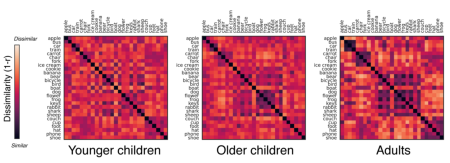
\includegraphics{figs/RSAAllCat-1} 

}

\caption[Category correlation matrixes in the highest layer of VGG-19 (FC7) for drawings made by younger children ( 3-6 years of age), older children (7-10 years of age), and adults (Google QuickDraw database)]{Category correlation matrixes in the highest layer of VGG-19 (FC7) for drawings made by younger children ( 3-6 years of age), older children (7-10 years of age), and adults (Google QuickDraw database). Each square in one of these matrixes represnets the correlation between two categories (e.g., chair and couch) in this layer of the network; lighter colors indicate higher correlations. Data-driven analyses were used to group the categories to reveal the similarity clusters. }\label{fig:RSAAllCat}
\end{figure*}
\end{CodeChunk}

\subsection{Results}\label{results-1}

We first compared the category similarities in the highest layer of the
network (FC7). Overall, we found that 3-5 year-old's drawings had
category similarities that only weakly resembled adults (Spearman's
r=.20), while 5-7 year olds had more apparent category similarities
(Spearman's r=.53), and 8-10 year olds had the highest similarities
(Spearman's r=.68), see Figure \ref{fig:RSAAllCat}). We found the same
pattern of results when only anlayzing the smaller subset of categories,
finding that younger children's category similarities moderately
resembled adults (Spearman's r=XX), while older children's category
similarities were significantly more structured and adult-like
(Spearman's r=.67). Similarily, a simple linear classifier applied to
the outputs of the final layer of VGG-19 could classify sketches made by
older children at XX\%, and sketches made by younger children XX\%
(adults=XX\% of the time).

Next, we examined the featural similarities between sketches produced by
adults and children at each layer of VGG-19, examining about the
layer-wise emergence of these similarites. For this analysis, we
restricted our comparisons to categogries for which we had three or more
drawings per category per age group. Overall, we found that the
similarity between children and adults' drawings increased in each
subsequent layer of the network, reaching a peak in the final layers of
the network (see Figure \ref{fig:layerWise}; Spearman's r values, Layer
1=0.215, ayer 1=0.206,Layer 3=0.249,Layer 4=0.435,Layer 5=0.637,Layer
6=0.696, Layer 7=0.72). For younger children, we found a similar pattern
of results, though similarity to adult drawings was overall lower
(Spearman's r values, Layer 1=0.074, Layer 2=0.001, Layer 3=0.04 , Layer
4=0.119, Layer 5=0.368, Layer 6=0.464, Layer 7=0.49). Thus, if anything
younger children's drawings were For older children. We again found the
same pattern of results when when analyzed only a subset of the
categories with a high number of drawings (younger children, peak at
layer XX, Spearman's r=XX; older children, peak at layer XX, Spearman's
r=XX). had fewer low-level features in commons with adults' drawings
than older children's drawings, suggesting that they in fact still
contained mid and high-level perceptual feature simialrities.

Taken together, these results suggest that children and adults are
accessing similar category representations to perform these drawing
tasks that manifest in perceptual similarities between adults and
children, even in the most primitive drawings.

\begin{CodeChunk}
\begin{figure}[H]

{\centering 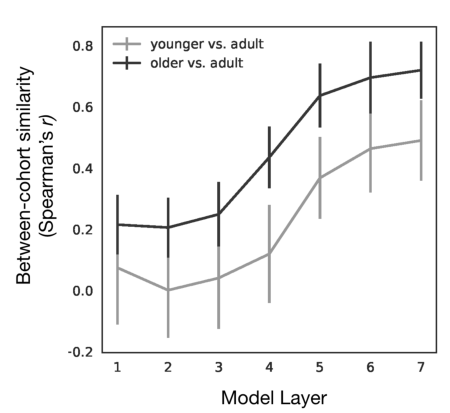
\includegraphics{figs/layerWise-1} 

}

\caption[Between-cohort similarity ]{Between-cohort similarity }\label{fig:layerWise}
\end{figure}
\end{CodeChunk}

\section{General Discussion}\label{general-discussion}

Overal, we found that the capacity to quickly produce graphical
representations that communicate object category information is highly
developed by middle childhood. Children produced drawings that were
recognizable by adults in under 30 seconds with only the few ``strokes''
of a pen. This work also points toward high-level similarities between
children and adults representations of object categories.

An obvious future direction for this work is to understand the
contribution of children's motor abilities in producing graphical
representations. In other words, to what degree are drawings made by
older children more recognizable simply because older children have
better fine motor control? Children certianly practice drawing
objects----both on their own and in structured settings (e.g., art
classes)--and this practice invariably plays a role in the fidelity of
the drawings that children can produce. In the future, we plan to
measure children's fine motor control on an orthogonal task (e.g.,
tracing a complex shape) to begin to understand how this factor
influences the recognizability of the drawings that children produce.

Ultimately, we seek to understand the degree to which changes in
children's drawings of objects reflect changes in children's
representations of object categories. In other words, one possibility is
that children's internal represntaitons of ``rabbit'', ``chair'', and
``couch'' are becoming more detailed as they grow older, and that it is
these more detailed representations that, in turn, feed into their rapid
drawings of these object categories. Throughout childhood, children
certainly acquire a wealth of experience with the objects in the world
around them, and this experience likely helps build more detailed
internal representations of the categories. If this is the case, then
children's abilities to depict certain object categories may patterns
with their object categorization errors. For example, are older
(vs.~younger) children both better able to draw cats vs.~rabbits and
better able to distinguish between cats vs.~rabbits? Future work that
links childrens perceptual and categorization abilities with their
production behaviors may begin to answet this question.

In sum, this work begings a developmental project examining childrens
internal object representaitons using a simple production task--drawing.
An understanding of how we form simple visual abstractions of the
objects in our everyday world is likely to help uncover the building
blocks of our category representations.

\section{Acknowledgements}\label{acknowledgements}

We gratefully acknowledge those who made the Google QuickDraw database
avaliable. This work was funded by a \#\# to Judy Fan, and a \#\#\# to
Michael C. Frank, and a \#\#\# to Bria Long.

\section{References}\label{references}

\setlength{\parindent}{-0.1in} \setlength{\leftskip}{0.125in} \noindent

\hypertarget{refs}{}
\hypertarget{ref-bloom1998intention}{}
Bloom, P., \& Markson, L. (1998). Intention and analogy in children's
naming of pictorial representations. \emph{Psychological Science},
\emph{9}(3), 200--204.

\hypertarget{ref-callaghan1999early}{}
Callaghan, T. C. (1999). Early understanding and production of graphic
symbols. \emph{Child Development}, \emph{70}(6), 1314--1324.

\hypertarget{ref-Efron:1979ts}{}
Efron, B. (1979). 1977 Rietz Lecture - Bootstrap Methods - Another Look
at the Jackknife. \emph{Annals of Statistics}, \emph{7}(1), 1--26.

\hypertarget{ref-fan2015common}{}
Fan, J. E., Yamins, D., \& Turk-Browne, N. B. (2015). Common object
representations for visual recognition and production. In \emph{CogSci}.

\hypertarget{ref-gardner1994arts}{}
Gardner, H. (1994). \emph{The arts and human development: With a new
introduction by the author}. Basic Books.

\hypertarget{ref-konkle2011canonical}{}
Konkle, T., \& Oliva, A. (2011). Canonical visual size for real-world
objects. \emph{Journal of Experimental Psychology: Human Perception and
Performance}, \emph{37}(1), 23.

\hypertarget{ref-Tukey:1958wn}{}
Tukey, J. W. (1958). Bias and confidence in not-quite large samples.
\emph{Annals of Mathematical Statistics}.

\end{document}
